\subsection{Grobplanung}
In der Grobplanung wurden die wichtigsten Meilensteine des Gesamtsystems und der einzelnen Disziplinen festgehalten.
Der Zeitstrahl in Abbildung \ref{fig:rahmenplanung} zeigt die chronologische Reihenfolge an. Als klar wurde, dass die Umsetzung in Verzug war, wurde die Planung angepasst. Vorallem im Bereich der Elektrotechnik wurde der Engpass ersichtlich. Wir waren uns bewusst, dass es dort zu Verzögerungen kommen kann, da dieser Bereich mehr oder weniger eine one-man-show ist. Darum wurden im ET Bereich zuerst Arbeiten erledigt, welche Abhängigkeiten mit anderen Disziplinen hatten.

\subsubsection{Stand 19.02.2015}
Der Rahmenplanung sind die wichtigsten Termine zu entnehmen. Dies sind drei offizielle Termine wie diverse kleinere, welche jeweils von den Disziplinen selbst für sich gesetzt wurden. Der erste Meilenstein wurde auf den 6. März datiert, dort soll sich das Team über die Planung und Umsetzung sicher sein.
Meilenstein zwei wurde auf den 10. April festgelegt, mit dem Ziel die Maschine fertig montiert zu haben. Eine Woche später sollte anschliessend die Tests beginnen. Die lauffähige und getestete Maschine und zugleich 80\% der Dokumentation bildeten zusammen Meilenstein 3.

\begin{figure}[h!]
	\centering
	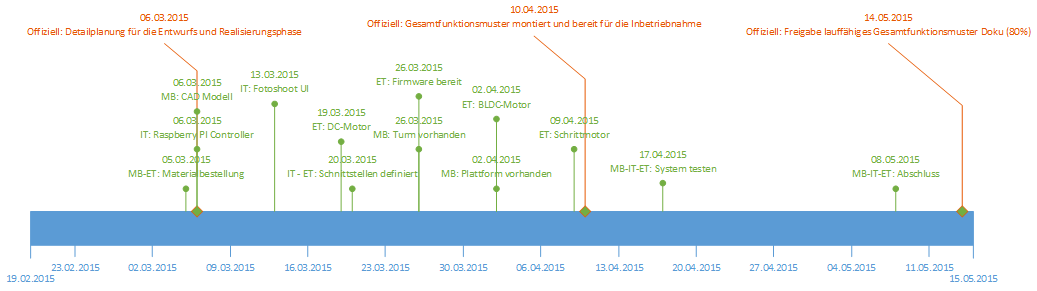
\includegraphics[width=1\linewidth]{../../fig/rahmenplanung}
	\caption{Rahmenplan vom 19.02.2015}
	\label{fig:rahmenplanung}
\end{figure}

\newpage
\subsubsection{Stand: 10.04.2015}
Am 10.04.2015 hat sich das Team zusammengeschlossen um über die restlichen Arbeiten zu diskutieren. Darauf hin hat man sich entschlossen die restliche Planung anzupassen. Nun wurden teilweise neue Termine definiert, welche für den restlichen Verlauf bindend sind.

\begin{figure}[h!]
	\centering
	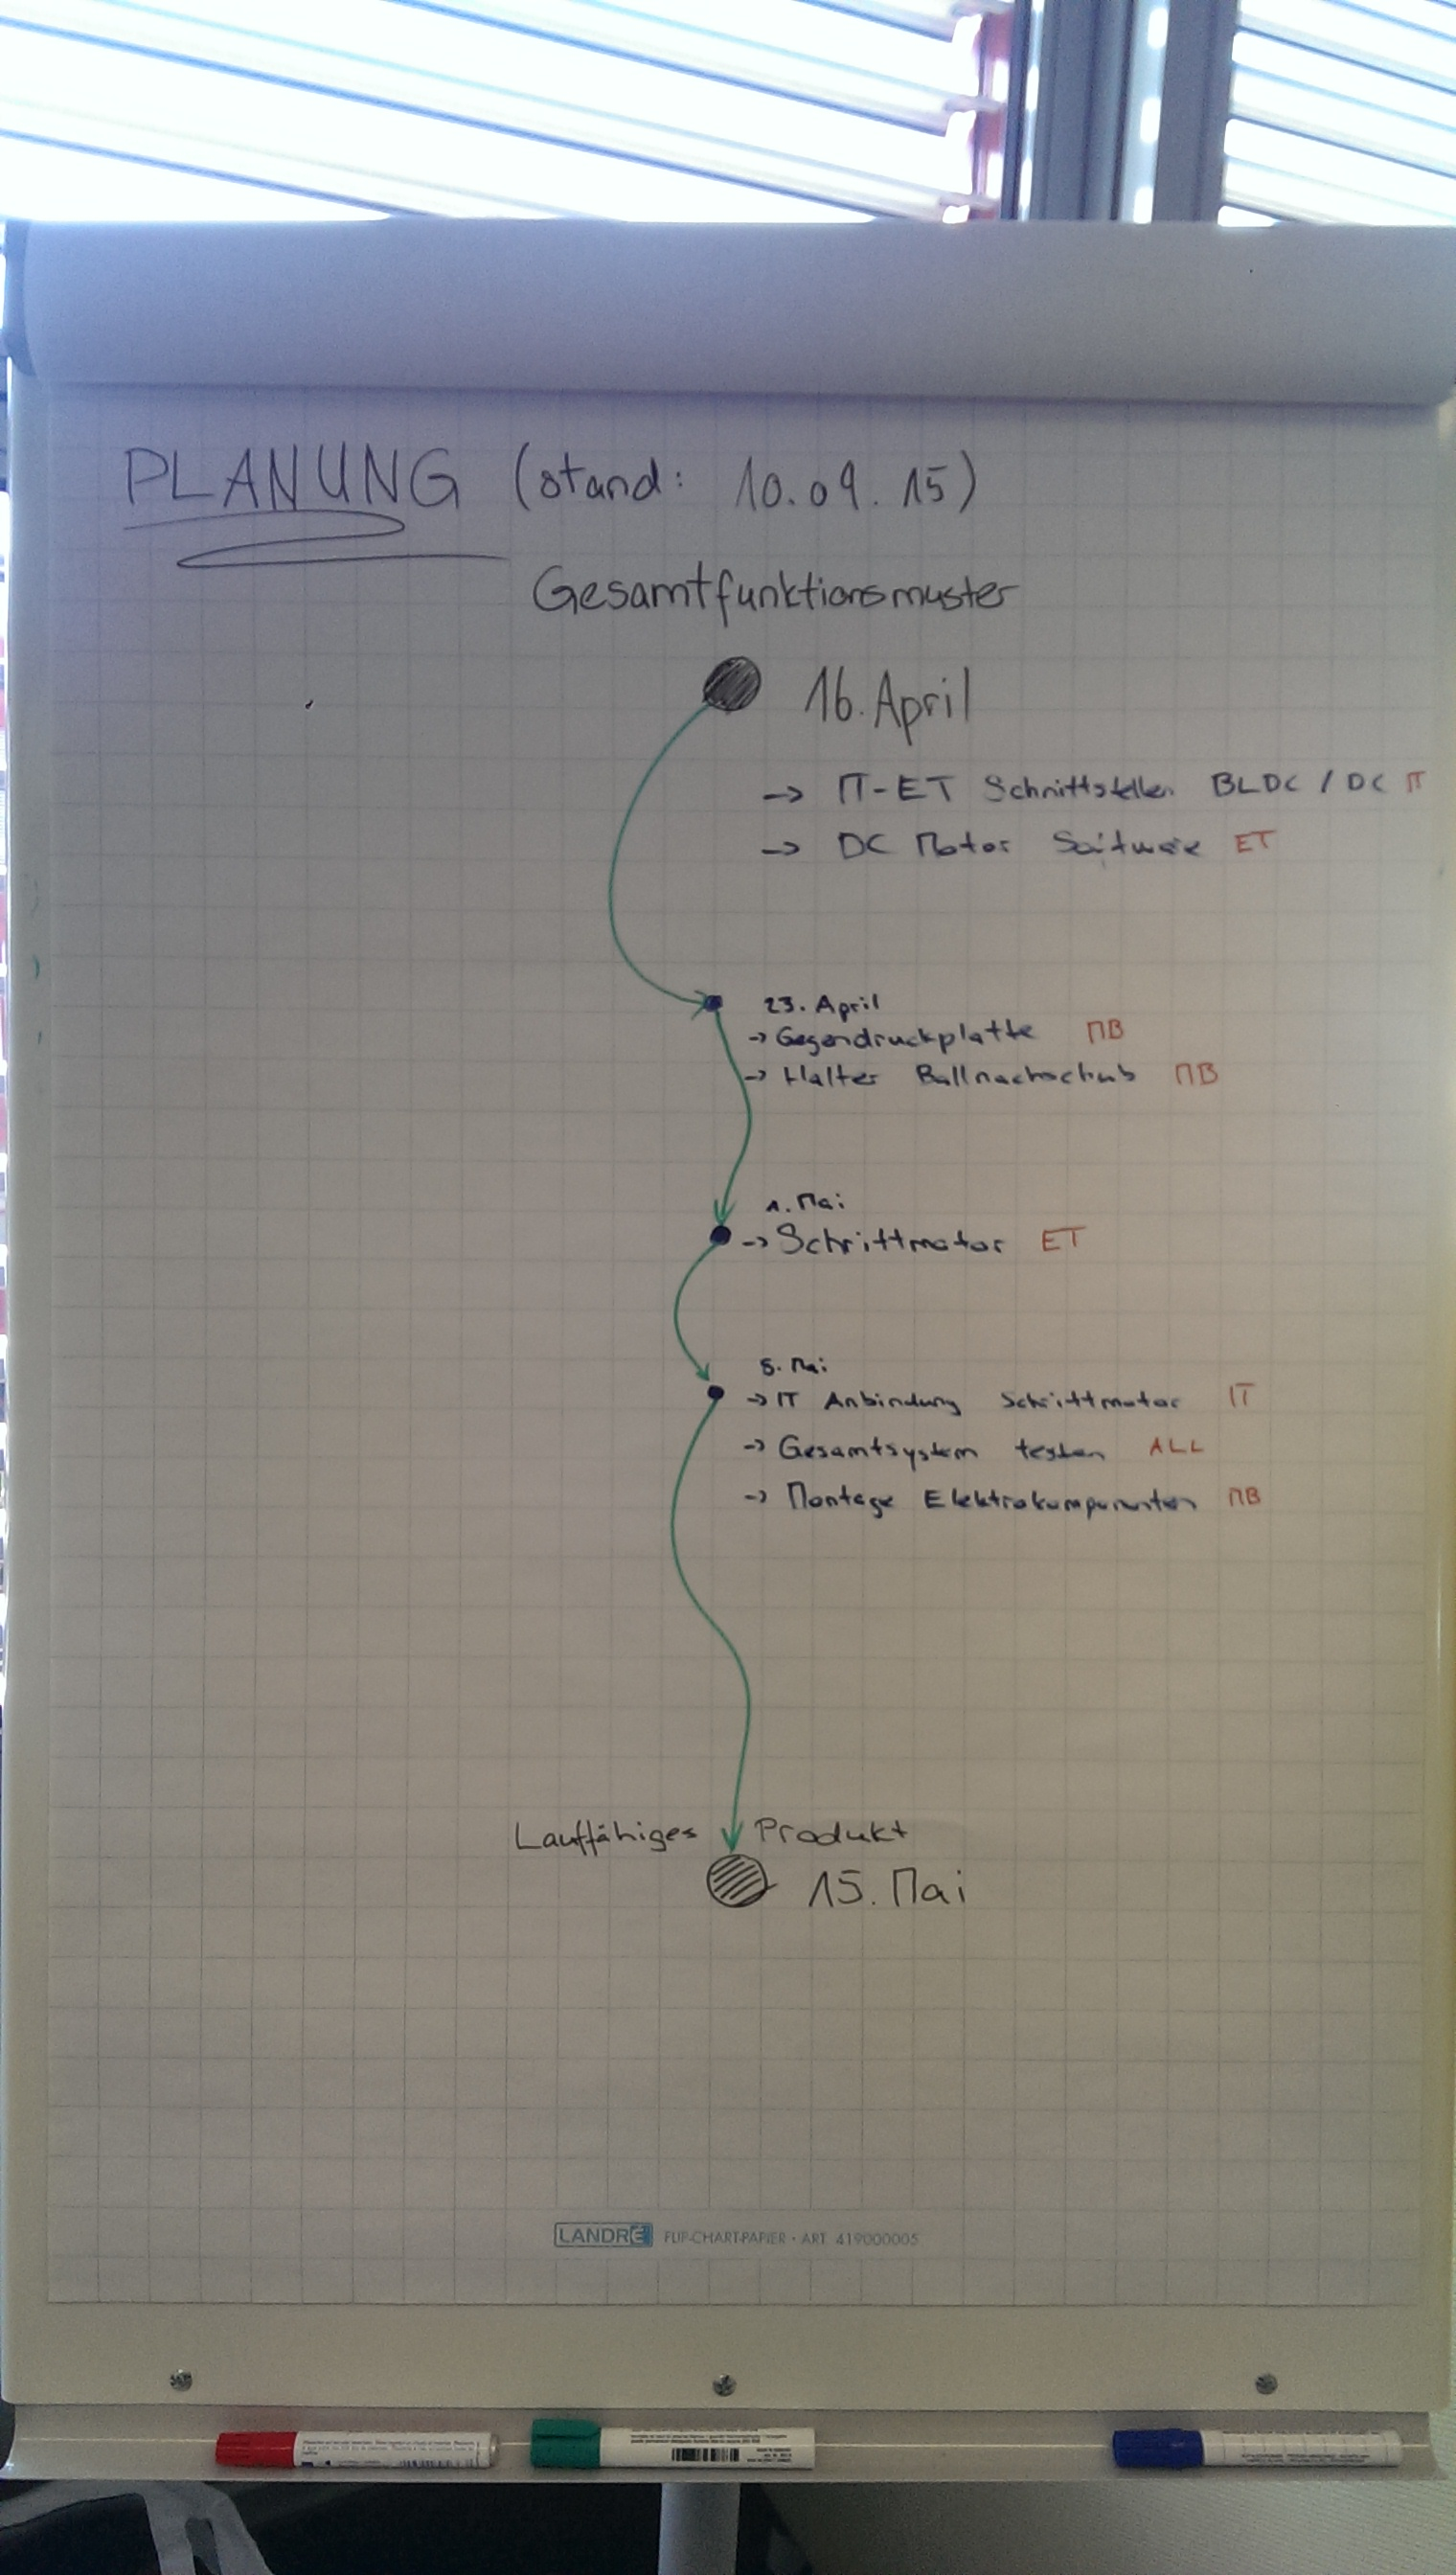
\includegraphics[width=0.6\linewidth]{../../fig/rahmenplanung-10042015}
	\caption{Rahmenplan vom 10.04.2015}
	\label{fig:rahmenplanung-10042015}
\end{figure}


